\documentclass[letterpaper]{article}
\usepackage[margin=1in]{geometry}
\usepackage{graphicx}

\usepackage{setspace}
\usepackage{natbib}
\usepackage{tabularx}
\usepackage{array}
\usepackage{hyperref}
\usepackage{breakurl}
\bibpunct{[}{]}{,}{n}{,}{,}

%\bibliographystyle{plainnat}
\documentclass[12pt]{article}
% \usepackage[margin=1in]{geometry}
% %\usepackage{mathptmx}
% %\usepackage[scaled=.90]{helvet}
% %\usepackage{times}
% \usepackage{setspace}
% \usepackage{natbib}


\begin{document}

\title{Natural Language Processing for Spoken Dialog Systems}
\author{Alex Sekula}
\date{\today}


\begin{document}
\maketitle

% explain the whole project
% The Boston Home
% Functions of the dialog system
\begin{abstract}
%Put in the abstract
\end{abstract}

\doublespacing

\section{Using Adaptive Boosting with Part-of-Speech Features} 
\subsection{Introduction}
	The speech recognizer on the robotic wheelchair has an error rate of 9\%. When it takes in an input sentence, it returns 10 hypotheses for what the input sentence was, with the first being one it is most sure of, the last being the hypothesis that the recognizer was least sure of. A test set was created by William Li to use to train the speech recognizer--residents at the Boston Home heard the input sentence and were asked to mark whether each hypothesis was correct or incorrect. Along with the sentence, different scores were taken based on a few features of the speech, including the acoustic score and language-model features. These features were then used by AdaBoost, an adaptive boosting algorithm, to train the classifier for future confidence scoring \cite{Schapire1995}. Splitting the past data set into a training set and test set enabled finding the error rate for the features used in AdaBoost. 
	The features used in AdaBoost were mostly audio features, meaning that they were taken from the input audio file. To find more features that would be trained in AdaBoost to get the confidence score, the outputted sentence could be parsed by the Stanford Parser to use the parts of speech as features.

\subsection{Approach}
	To decrease the error rate of the speech recognizer, NLP features can be extracted from the outputted text to. These features would then be used to classify whether the sentence is correct or incorrect. Also, these features could also be used to train the classifier using AdaBoost. To find these features, the Stanford Parser was used.
At first these features were analyzed to find grammatical features that were used to score how grammatical the input sentence was, but this did not have a beneficial result on the test set, because non-grammatical sentences were marked correct if they still recognized the important parts of the input sentence.
	Instead, we used the Stanford Parser to simply extract all features that it could from the input sentence, and run it through the classifier that was obtained from AdaBoost. 
	The features were returned in a tree of features, in which each node is used as a feature for the sentences to get as much data as possible from the parser. 
Once the number of features for each sentence was found, the iterations began. For each iteration, AdaBoost wanted to minimize the equation [INSERT EQUATION FROM TEXTBOOK AND EXPLAIN IT (VARIABLES)]. The base classifier $y_{m}$ was the feature count chosen to train the final classifier. The count of each feature was used to separate the correct and incorrect sentences, and the feature count that was most accurate was chosen. Then, the weights were updated to make sure that the stronger classifiers were counted more. [EXPLAIN THE WEIGHT UPDATING].
Each classifier matched with their weight trained the final classifier, which was used on the test set to find how well it performed.

\subsection{Results}
	The test set used was a set of around 25,000 sentences that were generated by residents at The Boston Home. They were asked to say sentences, then go through each of the 10 hypotheses and mark whether it was correct or incorrect. This massive test set was split into 80-20 training-test sets. 80% of the sentences were used to train the classifier, and then 20% percent were used to test how well the features trained the classifier. 
The training and test sets are taken randomly, but the probabilities were usually within 2 percent of each other. Also, in AdaBoost the number of features that are used to train the classifier changes the score, with the greater number of features improves the success rate, reaching an asymptote. 
A graph showing the classifier created by AdaBoost from the training set is show below. It was tested on both the training set and test set to show the relation. Also, the grammatical features used in the classifier is shown as well. 

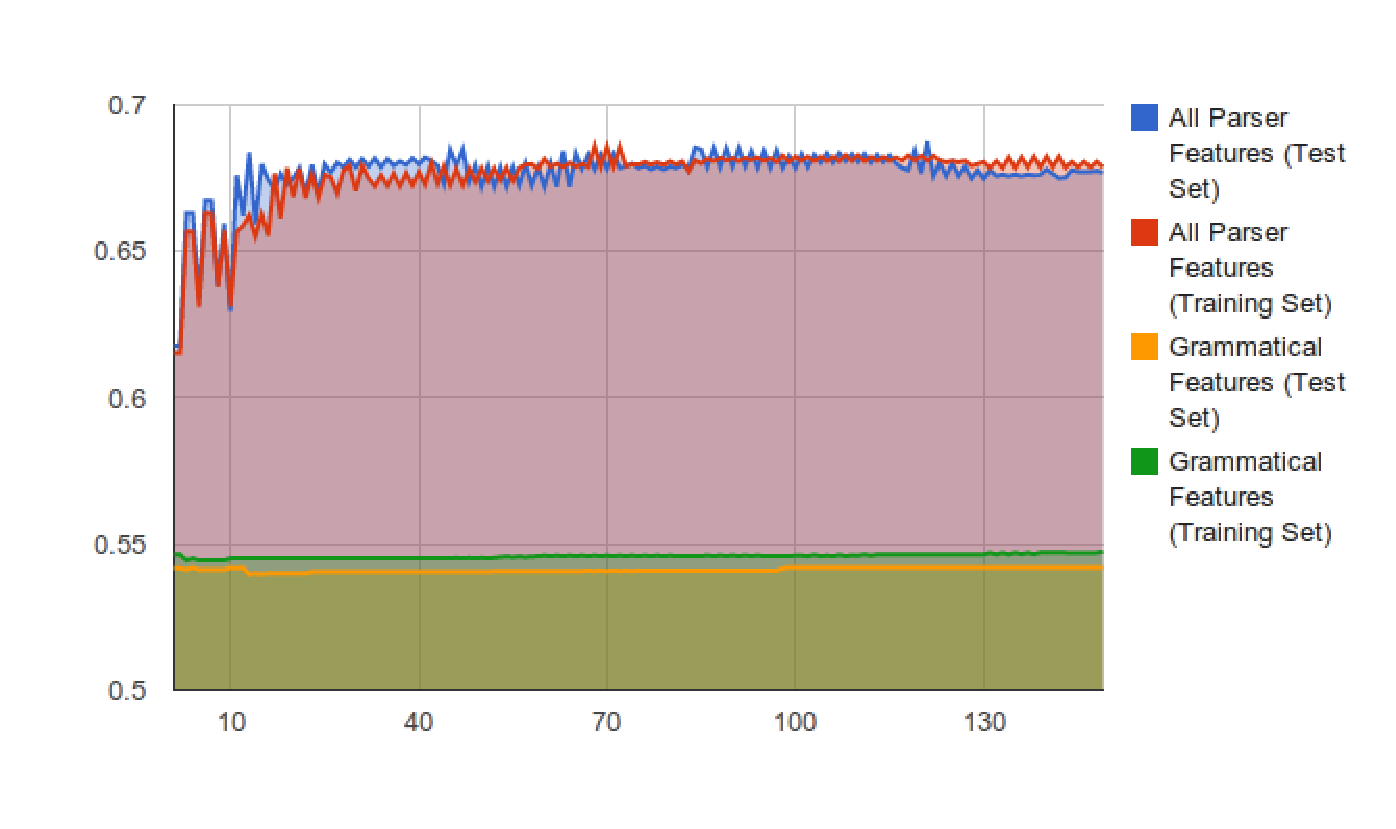
\includegraphics[width=120mm]{figs/AdaBoost_Graph.eps}

A table with the percentages after 150 iterations of AdaBoost are shown below.
\begin{table}
    \begin{tabular}{|l|l|l|}
        \hline
        ~            & All Parser Features & Grammatical Features \\ \hline
        Training Set & 67.8                & 54.7                 \\ 
        Test Set     & 67.7                & 54.2                 \\
        \hline
    \end{tabular}
\end{table}
Notice how the simpler feature extraction does significantly better, and the variety of beneficial features is shown by the curve of the increase iterations of AdaBoost. This curve indicates that as AdaBoost runs more iterations, newer features are added to the classifier, improving it. The lack of a curve of the grammatical features shows how a relatively small amount of features were used to train the classifier, showing how the grammatical features were either not implemented correctly, or simply not useful.
Not all features from the Stanford Parser were used, only the ones that actually benefitted the classifier were used. The features that were used by AdaBoost in order are shown below:

S, NNS, JJR, WHPP, SBAR, WHADJP, SBAR, WHADJP, NNS, S, WDT, VBD, RBR, QP, NN, WHADJP, X, NP, UH, QP, DT, SBAR, SBAR, WHADJP, NNP, X, WP, NN, WHADJP, DT, NNS, PRN, QP, SBAR, NNS, WHADJP, DT, QP, DT, WP, X, VBD, DT, WP, DT, NNP, S, NNS, DT, PRP\$, DT, WP, DT, QP, S, NP, X, SBAR, DT, WP, DT, VBD, UH, QP, NN, WP, DT, SBAR, DT, WP, X, WP, DT, JJ, RB, VBD, DT, NNP, CD, WP, DT, QP, S, ADJP, S, JJ, PRN, NNS, DT, NNP, S, JJ, PRN, JJ, WHADJP, SBAR, VBD, NN, NP, RB, NNP, DT, VB, WHADJP, WP, DT, NNP, WHADJP, VBD, NNS, RRC, VB, WHADJP, QP, DT, NNP, RB, PRP\$, X, VB, WHADJP, SBAR, WHADJP, WP, DT, VB, DT, JJ, WHADJP, NNP, DT, WP, WHADJP, VB, DT, VBZ, SBAR, VBD, X, NNP, WHADJP, VBD, WHADJP, WP, DT, VB, NNS, PRN, NNS, S

A description of each tag in the Stanford Parser can be found here:

\verb+http://www.ldc.upenn.edu/Catalog/desc/addenda/LDC1999T42/TAGGUID1.PDF+

\section{Language Understanding through Web-Based Word Association}
\subsection{Introduction}
The dialog system that was used to understand input sentences was very simple. The baseline approach simply used a keyword extractor to determine the mapping of speech hypotheses to concepts. For example, if an input sentence contained both the words ``weather'' and ``tuesday'', then the dialog system would show the weather for tuesday. In order for a category to be chosen, both words of the category must be inside the input sentence. There is a major flaw in this approach, because if an input sentence was “what is the forecast for tuesday'', or ``what are we eating tomorrow morning'' rather than ``what is breakfast tomorrow'', the dialog system would not be able to recognize the input. 

The goal of this part of the research was to find a way for the dialog system to associate words like ``forecast'' or ``rain'' with ``weather.'' As a result, if someone asks ``will it rain on friday'', it would be able to show the weather for friday, working as intended. This word association would work on top of the keyword searching, prioritizing the keyword searching, as to not alter any performance from the past but only enlarge the input possibility. By expanding the possible vocabulary that the system can understand, users can be less constrained and ask more natural queries to the dialog system.

\subsection{Approach}
	For each category, e.g ``weather today'', there are two sub-categories, e.g. ``weather'', ``today''. We need to do word associations on both sub-categories to find out how relevant the input sentence is to the category as a whole.


\textbf{Wikipedia Articles for Word Association: } To associate words like ``rain'' and ``forecast'' with ``weather'', we require a set of words that directly relate to ``weather'', but a broader relation rather than a simple definition. As a first step, we decided to scan Wikipedia articles to get a set of words that relate to each sub-category. This would be effective because the words in the Wikipedia article directly relate to the sub-category, because they are used to give information about this sub-category.

A limitation that was found with Wikipedia is that there was not always a Wikipedia article that directly corresponded to each sub-category. For example, a Wikipedia search for ``today'' would result in many different options, including TV shows and bands, so the Wikipedia article ``Present'' needed to be used for that sub-category. This would make expanding more difficult, because each sub-category would need to be manually checked whether the wikipedia article contains an entry that accurately relates to the sub-category.
The scanning was done with python’s urllib module, and a closer look at Wikipedia article source code showed that the article and all of the relating words are stored in \verb+<p>+ tags. These words are the ones that are to be associated with the sub-category.

% \begin{verbatim}
% Now I can finally write anything I want in LaTeX.
% \end{verbatim}

The only exceptions for the files are the days of the week, in which there is really only one way to say ``thursday''. Therefore, scanning articles relevant to thursday would not be very helpful.
Once the articles for each sub-category are scanned, a file containing the set of words is created, ending up with a whole set of files for each sub-category. Then, when we have the input sentence, to find the category that best matches that sentence, we applied the term frequency-inverse document frequency method described below \cite{Salton1988}. 

\textbf{Term Frequency-Inverse Document Frequency (tf*idf): } tf*idf is an expression used to find the relevance of a given word, $t$, to a certain document $d_n$ in a set of documents $D = {d_1, d_2, d_3 \ldots }$.  

The algorithm can be described as follows:
\begin{enumerate}
\item For a certain document, the term frequency $tf$ is calculated. The term frequency $tf$ for term $t$ in document $D$ is  $\frac{c(t)}{C}$, where $c(t)$ is the number of occurrences of $t$ in $D$ and $C$ is the total number of words in $d$.
\item The inverse document frequency $idf$, which takes the $log_{10}(\frac{|D|}{|\left d \in D : t \in d \right |})$.
\item The term frequency $tf$ is multiplied by the inverse document frequency to obtain the tf*idf score.
\end{enumerate}

For our language understand application, the goal is to determine which category produces the highest tf*idf score. Therefore, we compute the tf*idf score for each of the different categories for each of the terms in the input sentence. The sum of the tf*idf for each word in the input sentence to each document in the set of sub-category documents is used to find the relevance of the input sentence to each sub-category. By adding the two scores for each sub-category, we can find the score for each category.

\textbf{Combining Keyword Extraction with Web-Based Word Association: } However, in order to make sure that ``activities wednesday'' actually shows the activities on wednesday, the keyword searching must be prioritized in the ranking of categories. To do so we searched the sentence for any sub-categories that it might contain, and added a score that is higher than the maximum possible score ($maxscore = log_{10}(total number of documents)$ ) which would bring all categories that contain ``wednesday'' up higher, and bring the category ``activities wednesday'' up to the highest, overriding the tf*idf scores.

Specifically, we added 1000 to any score that contained a sub-category, with a maximum score being a bit higher than 2000. In some cases, like in ``show\_contacts'', each sub-category has multiple parts, separated by a ‘\_’. To address this issue, each word in the sub-category was searched, and 1000/total words in the sub category was added to the score. However, this would give ``system go\_to\_sleep'' an advantage, and when asked ``what are we going to eat tonight'', it would return ``system go\_to\_sleep'' with a score around 333 because of the ``to''. To avoid this, only words with lengths greater than three characters were used in the keyword searching.  To get a better sense of how well the word association was, we seeked different sources rather than just Wikipedia articles. Wikipedia provided a formal description of words, so we searched for a different source of words that would provide a more colloquial use of words to find different word associations.

\textbf{Scanning Tweets for Word Association: }The next source that we used to get a word set for each sub-category was Twitter. The Twitter Search API was used to scan tweets that contained the word of the sub-category, and the words inside the tweets were used as the word set for each sub-category. The use of Twitter had a few benefits: Expanding the number of sub-categories would be easy, because they are used in the search, and a lot more data could be used because it returned as many tweets as desired.\footnote{Due to the long time that it would take to scan all the tweets that contain each sub-category, only 1000 tweets were used per sub-category.}

To scan the tweets, multiple calls were made to the url:

\verb+http://search.twitter.com/search.atom?q=keyword&rpp=100&page=pagenum+

%make this a enumerate list
 ``Keyword'' was replaced by each sub-category, and pagenum went from 1 to 10, which indicated the number of the page returned. The body of each tweet was returned inside a \verb+<title>+ tag in the xml returned, and using python and urllib the words were stripped from the returned page and put into files for each sub-category.

After the files for the twitter word set were made, tf*idf was used again for the new word association.

\textbf{Word Associations from the Crowd: Amazon Mechanical Turk: }A third and final word set that we got was from the AMT (Amazon Mechanical Turk). To get both a test set and a word set for training the word association, we obtained a word set from the Amazon Mechanical Turk.

To get a word set that actually benefitted the word association, we asked people to type in how they would ask for a category without using the words of either category (e.g ``How would you ask for the breakfast menu without using the word ‘breakfast’?'' An example response from this prompt was ``What are we eating this morning?''). This could be more relevant to the word association because it could give us a chance to use actual sentences that people would ask to train the association. This also gave us a good test set to work with to test how well the Wikipedia and Twitter word sets performed, but there were some problems with it too (see Results). The input sentence words from the AMT were then put into files for each sub-category again, and once again tf*idf was used to train the word association.

The AMT had the most limitations from the three data sets, for a few reasons. These reasons included costing money, needing to wait over a few days for enough data, and not having close to as much data as the online sources did. However, the sentences retrieved from the AMT were the best because they mostly related directly to the categories.
For the dialog system, once the input sentences are scored, they will be used to increase or decrease each probability of each category in the dialog system. When an input sentence in the speech recognizer is recognized, each category is given a probability of how certain it is that the input sentence was asking for that category. In order for the scores to be incorporated in case the categories are not able to be found, the scores will be mixed in with the probabilities. Also, the dialog manager uses the POMDP method for choosing a category, and if two categories have very close scores, and if the higher one was rejected, then the second one could be asked to save time rather than having the user repeat the whole sentence.
 
\subsection{Results}
	To find results of the three methods of word association, two test sets were used. Both test sets contained questions for each category.
	One of the test sets was the one taken from AMT, and consisted of sentences that were created specifically so that none of the sub-categories were in any of the input sentences. This would cause the keyword searching to have an success rate of 0\% because it depended solely on the sub-categories being located inside of the sentence. However, since there was unfiltered data, the keyword searching has a success rate of around 10\%.
	The other test set was a one I personally created at the beginning of the year. I wrote down five to ten different ways that I would ask for each sub-category. Since this was at the beginning of the year before we started our project, the test set is not biased. The difference, however, is that there were no restrictions on the input sentence, and the sub-categories could be used in the sentence. This caused the keyword searching to already have roughly a 70% success rate.
	A table showing the scores for the data source on each test set is shown below.
\begin{table}
    \begin{tabular}{|l|l|l|l|l|}
        \hline
        ~             & Keyword Searching & Wikipedia & Twitter & AMT  \\ \hline
        My Commands   & 69.1              & 79.5      & 76.1    & 74.9 \\ 
        Turk Commands & 9.9               & 37.4      & 23.5    & 63.0 \\
        \hline
    \end{tabular}
\end{table}
% Explain the able

There are still some errors with the test sets. The test set created by me does not have too much data to test upon, and most of the success of the methods on that training set was because of the keyword searching. The AMT test set also has a few flaws. When under the restrictions for the input sentences, the users got creative and sentences like ``will we play cards later''. This resulted in much lower scores than the other test set.

\subsection{Further Work}
	To improve the word association, other sources could be used. For example, data directly from The Boston Home residents could be taken and used to train the word association. This would have the best effect on the dialog system because the data taken was exactly the data needed to have classified the sentence correctly. 
	Other sources considered that will have different effects on the system would be a dictionary and a thesaurus. These might have a beneficial effect on the system, but the main focus was to find ways to associate words that are related, not words that essentially have the same meaning.
	Another improvement that could be done to the system that would get really deep into Natural Language Processing would be to search for words using conjugated or different forms (like plural) of the word in the sentence. For example, if someone said ``i like to eat today'', and a the Wikipedia articles for breakfast, lunch, and dinner contained the word ``eating'', not ``eat'', the association would not be made. Searching the files with different forms of the words in the sentence would potentially increase the success rate, improving the overall success of the dialog system.



\newpage
\bibliographystyle{plainnat}
\bibliography{references}
\end{document}

